\documentclass[border=10pt]{standalone}
\usepackage{tikz}
\usetikzlibrary{arrows.meta, positioning, patterns}

\begin{document}
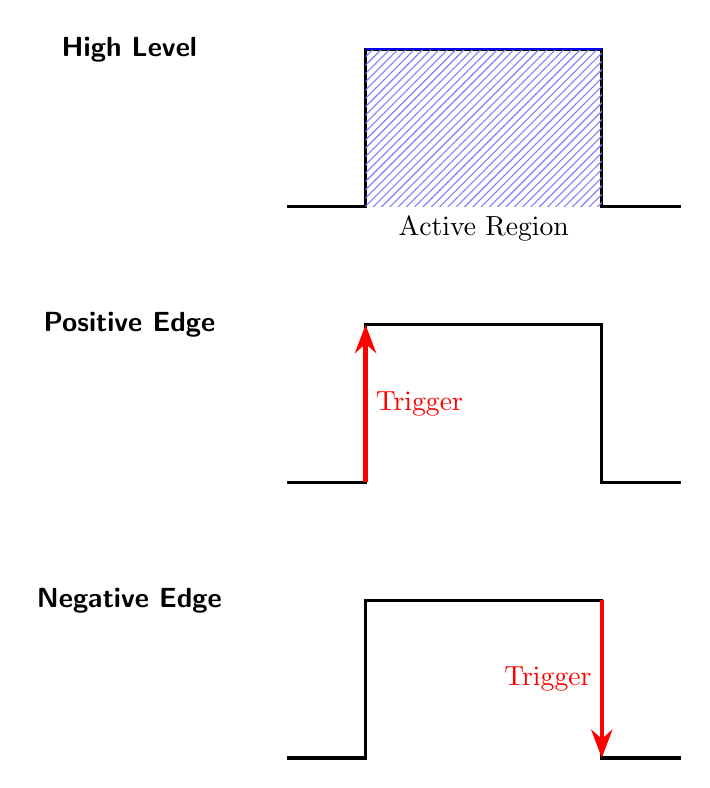
\begin{tikzpicture}[
    thick,
    >=Stealth,
    node distance=1.5cm,
    pulse/.style={draw, very thick},
    label_text/.style={font=\sffamily\bfseries}
]

    % === 1. High Level Triggering ===
    \node[label_text] (lbl1) at (-2, 2) {High Level};
    
    % Draw Clock Pulse
    \draw[pulse] (0, 0) -- (1, 0) -- (1, 2) -- (4, 2) -- (4, 0) -- (5, 0);
    
    % Highlight High Level
    \fill[pattern=north east lines, pattern color=blue!50] (1, 0) rectangle (4, 2);
    \draw[blue, thick] (1, 2) -- (4, 2);
    
    % Labels
    \node[below] at (2.5, 0) {Active Region};
    
    
    % === 2. Positive Edge Triggering ===
    \node[label_text] (lbl2) at (-2, -1.5) {Positive Edge};
    
    \begin{scope}[yshift=-3.5cm]
        \draw[pulse] (0, 0) -- (1, 0) -- (1, 2) -- (4, 2) -- (4, 0) -- (5, 0);
        
        % Highlight Rising Edge
        \draw[red, ultra thick, ->] (1, 0) -- (1, 2);
        \node[right, red] at (1, 1) {Trigger};
    \end{scope}

    % === 3. Negative Edge Triggering ===
    \node[label_text] (lbl3) at (-2, -5) {Negative Edge};
    
    \begin{scope}[yshift=-7cm]
        \draw[pulse] (0, 0) -- (1, 0) -- (1, 2) -- (4, 2) -- (4, 0) -- (5, 0);
        
        % Highlight Falling Edge
        \draw[red, ultra thick, ->] (4, 2) -- (4, 0);
        \node[left, red] at (4, 1) {Trigger};
    \end{scope}

\end{tikzpicture}
\end{document}
